% !TEX root = BA-Bauer.tex
\subsection{Einstellungen}
Dem Benutzer soll die Möglichkeit gegeben werden, bestimmte Anpassungen am Gerät vorzunehmen, um die Funktionsweise und Eigenschaften des Gerätes auf die eigenen Bedürfnisse anzupassen. In den folgenden Kapiteln wird auf die Einstellungsfunktionen eingegangen und deren Funktionsweise erläutert.
\subsubsection{LCD-Kontrast \& LED-Helligkeit}
Das Gerät kann durch die zahlreichen Einsatzgebiete auch an vielen verschiedenen Orten eingesetzt werden. Um zu garantieren, dass die auf dem LCD-Display angezeigten Inhalte jederzeit erkennbar sind, soll der Benutzer die Möglichkeit haben den Kontrastwert des Displays einzustellen. Gleiches gilt für die Helligkeit der LEDs. Soll das Gerät an einem unauffälligen Ort platziert werden, könnten aufblinkende LEDs stören. Aus diesem Grund sind die Einstellungsfunktionen zum Einstellen des LCD-Kontrastes und der LED-Helligkeit implementiert. In diesem Kapitel wird auf das Prinzip beider Funktionen eingegangen. Beide Einstellungen basieren auf dem gleichen Prinzip, der PWM-Steuerung. \\
\newline
\textbf{LCD-Kontrast}\\
In der Regel wird mithilfe eines einstellbaren Spannungsteilers (Potentiometer) eine Spannung an den $V0$-Pin des LCD-Moduls angelegt und damit der Kontrast geregelt. Diese verschiedenen Spannungswerte können auch mithilfe eines PWM-Signals erzeugt werden. Abbildung \ref{fig:lcdk25}, \ref{fig:lcdk50} und \ref{fig:lcdk75} zeigen die Auswirkungen der Änderung der Pulsweite auf den Kontrast des LCD-Displays. 
\begin{figure}[h]
	\begin{minipage}{.3\linewidth}
		\centering
		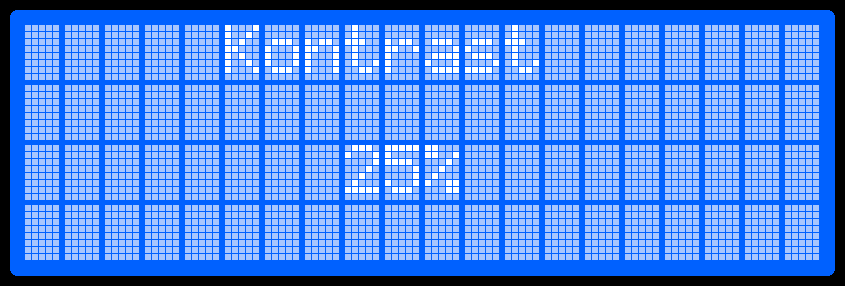
\includegraphics[width=\linewidth]{LCD-Screenshots/LCDKontrast25}
		\caption{LCD 25\% Kontrast}
		\label{fig:lcdk25}
	\end{minipage}
	\hfill
	\begin{minipage}{.3\linewidth}
		\centering
		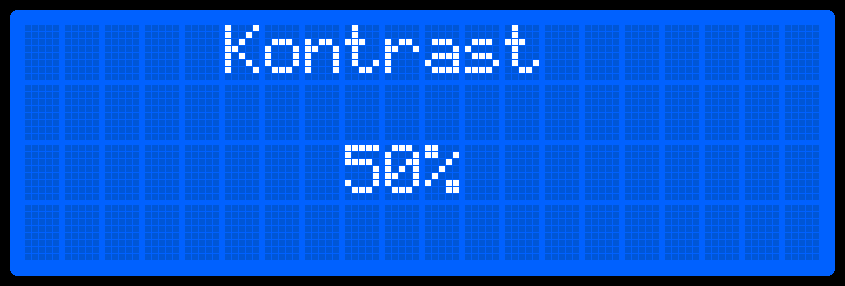
\includegraphics[width=\linewidth]{LCD-Screenshots/LCDKontrast50}
		\caption{LCD 50\% Kontrast}
		\label{fig:lcdk50}
	\end{minipage}
	\hfill
	\begin{minipage}{.3\linewidth}
		\centering
		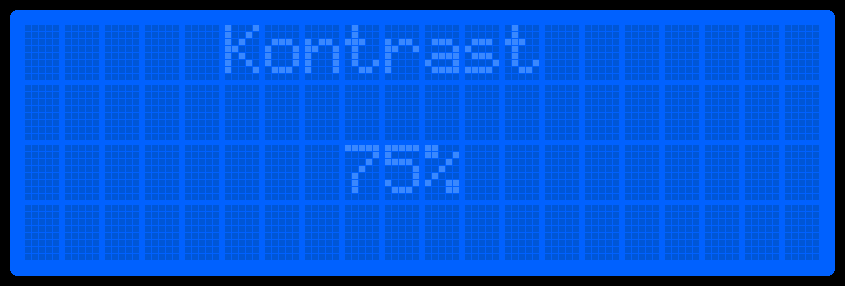
\includegraphics[width=\linewidth]{LCD-Screenshots/LCDKontrast75}
		\caption{LCD 75\% Kontrast}
		\label{fig:lcdk75}
	\end{minipage}
	\hfill
\end{figure}
Der Kontrastwert wird mithilfe des Encoders verändert und wird entsprechend auf dem Display angezeigt. Der Wert wird bei einer Drehbewegung im Uhrzeigersinn erhöht und bei einer Drehung gegen den Uhrzeigersinn verringert.\\
Für die Erzeugung des PWM-Signals wird Timer 1 des MCUs verwendet, welcher mit einer Frequenz von 10\,kHz Pulse an einem Ausgangspin erzeugt, der mit dem $V0$-Pin des LCD-Moduls verbunden ist. Die Pulsweite wird durch das Beschreiben des $CCR$-Registers\footnote{Capture Compare Register} mit Werten von 0-100 eingestellt. In der Einstellungsfunktion entspricht der Wert des $CCR$-Registers dem Kontrastwert in \%. Das Signal des Ausgangspins des Timer wird in Abbildung \ref{fig:PWM25} mit einer Pulsweite von 25\%, in Abbildung \ref{fig:PWM75} mit einer Pulsweite von 75\% gezeigt. 
\begin{figure}[h]
	\begin{minipage}{.48\linewidth}
		\centering
		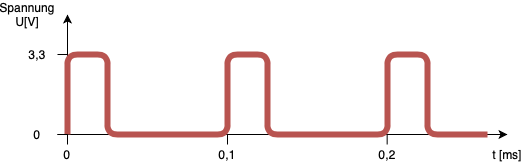
\includegraphics[width=\linewidth]{PWM25}
		\caption{10\,kHz PWM-Signal mit 25\% Pulsweite}
		\label{fig:PWM25}
	\end{minipage}
	\hfill
	\begin{minipage}{.48\linewidth}
		\centering
		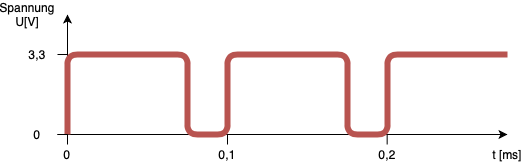
\includegraphics[width=\linewidth]{PWM75}
		\caption{10\,kHz PWM-Signal mit 75\% Pulsweite}
		\label{fig:PWM75}
	\end{minipage}
\end{figure}
\\
\newline
\textbf{LED-Helligkeit}\\
Wie auch der Kontrast des LCDs wird die Helligkeit der LEDs mithilfe eines PWM-Signals eingestellt. Für die LEDs wird Timer 9 des MCUs mit einer Pulsfrequenz von 12,5\,kHz verwendet. Bei dieser Frequenz ist bei niedrigen Helligkeiten kein Flackern der LEDs zu erkennen. Um den Effekt der Einstellung sichtbar zu machen, wird eine LED während der Einstellungsfunktion eingeschaltet. Die Einstellung der LED-Helligkeit unterscheidet sich von der Einstellung des LCD-Kontrasts lediglich in der auf dem LCD-Display angezeigten Überschrift und durch die Verwendung eines anderen Timers und zu beschreibenden Registers.
\subsubsection{NPC ändern}
Das Zeichen, welches in der Aufnahmedatei zum Signalisieren des Datenpaketendes genutzt wird (NPC-Zeichen), ist initial 1. Die eingehenden DMX-Datenpakete werden während der Aufnahme nach diesem Zeichen durchsucht und durch ein anderes Zeichen (0) ersetzt. In speziellen Fällen wird das NPC-Zeichen explizit für die Steuerung von DMX-Geräten benötigt. Um eine Aufnahme der Daten und eine vollständig kompatible Wiedergabe der Daten trotzdem zu ermöglichen, hat der Benutzer die Möglichkeit das NPC-Zeichen und das entsprechende Ersatzzeichen frei zu wählen. 
\begin{figure}[h]
	\begin{center}
		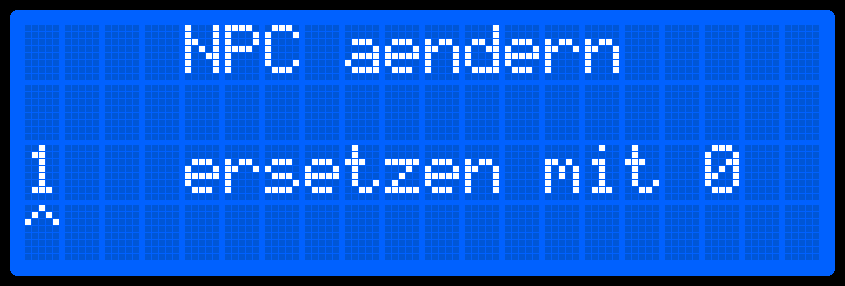
\includegraphics[width=.3\linewidth]{LCD-Screenshots/NPC}
		\caption{LCD-Ausgabe NPC Einstellung}
		\label{fig:npc}
	\end{center}
\end{figure}
Abbildung \ref{fig:npc} zeigt den Inhalt des LCD-Displays der NPC-Einstellungsfunktion. Das Zeichen in der untersten Zeile des Displays signalisiert die aktuelle Auswahl und kann mit den Links- und Rechts-Tastern verändert werden. Der ausgewählte Wert wird mit der Drehung des Encoders eingestellt. Ist eine Auswahl getroffen, muss sie mit dem Bestätigen-Taster bestätigt werden. Daraufhin wird überprüft, ob beide Werte unterschiedlich sind. Sind beide Werte identisch, wird eine Fehlermeldung über das LCD-Display ausgegeben. Andernfalls werden die Werte gespeichert und die Funktion kehrt zum Menü zurück. Die Funktion kann zudem jederzeit durch die Betätigung des Zurück-Tasters beendet werden.
\subsubsection{Trigger}
Um eine $Trigger$-Aufnahme zu starten muss ein $Trigger$-Wert eines bestimmten $Trigger$-DMX-Kanals überschritten werden, wie in Kapitel \ref{sec:recfunctions} erläutert ist. Um dem Benutzer auch hier die Möglichkeit einer Personalisierung zu geben, sind der $Trigger$-Kanal und -Wert vom Benutzer in den Einstellungen frei wählbar. Dadurch kann der Benutzer die Adressen der DMX-Geräte ohne Einschränkungen vergeben und anschließend einen entsprechenden freien Kanal für die $Trigger$-Funktionalität in den Einstellungen auswählen. 
\begin{figure}[h]
	\begin{center}
		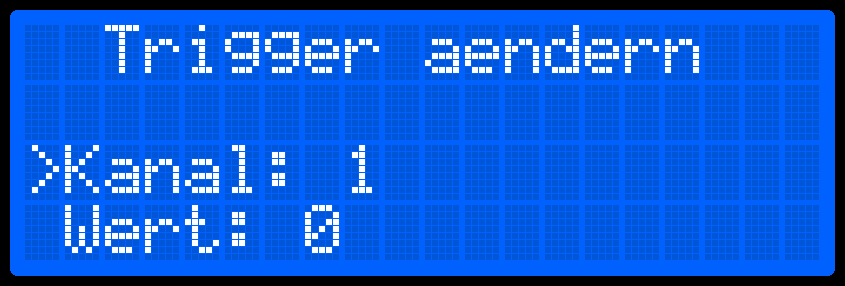
\includegraphics[width=.3\linewidth]{LCD-Screenshots/Trigger}
		\caption{LCD-Ausgabe Trigger-Einstellung}
		\label{fig:trig}
	\end{center}
\end{figure}
Abbildung \ref{fig:trig} zeigt die Ausgabe der Trigger-Einstellungsfunktion auf dem LCD-Display. Ein Zeichen in der ersten Spalte des LCD-Displays zeigt die aktuelle Auswahl an. Der Kanal bzw. der Wert wird durch Drehen des Encoders verändert. Es können Kanäle im Bereich von 0 bis 512 und Werte im Bereich von 1 bis 255 eingestellt werden. 
\subsubsection{Aufnahme löschen}
In dieser Einstellungsfunktion hat der Benutzer die Möglichkeit Aufnahmen zu löschen. Die Funktion durchsucht zunächst die SD-Karte nach Dateien mit der Endung $.dmx$ und zeigt deren Namen auf dem LCD an. Durch drehen des Encoders kann die zu löschende Datei ausgewählt werden, welche mit einem vor dem Dateinamen befindlichen Pfeil angezeigt wird. Für die Auswahl der Datei wird dieselbe Funktion verwendet, die in der Wiedergabefunktion Anwendung findet (Kapitel \ref{sec:selectfile}). Wird die Auswahl mit dem Bestätigen-Taster bestätigt, wird der Benutzer durch eine entsprechende Anzeige auf dem LCD zum Bestätigen des Löschvorgangs aufgefordert. Wird auch diese bestätigt, wird die entsprechende Aufnahme- und zugehörige Info-Datei gelöscht. Wird jedoch der Zurück-Taster betätigt, kehrt die Funktion zum Menü zurück. Der Löschvorgang wird mit der Funktion $f\_unlink()$ der FATFS-Bibliothek durchgeführt. Die Daten werden dabei nicht gelöscht, sondern lediglich die entsprechenden Speicherplätze wieder freigegeben, also aus der Dateizuordnungsliste des Dateisystems entfernt.